%
% Optional reading
%

\begin{frame}[plain,c]
\begin{center}
{\Huge \bf Optional reading for Lecture \thislecture}
\end{center}
\end{frame}


%
%
%

\begin{frame}{The electrostatic potential energy is stored in the field}

We can now prove a statement I made earlier: That {\bf the electrostatic potential energy is stored in the electric field}.\\
\vspace{0.1cm}
The potential energy stored in a system of N charges can be written as:
\begin{equation*}
   U = \frac{1}{2} \sum_{i,j=1;i{\ne}j}^{N} \frac{q_i q_j}{4\pi\epsilon_0|\vec{r}_{ij}|}
     = \frac{1}{2} \sum_{i}^{N} q_i {\color{red}\sum_{j=1;j{\ne}i}^{N} \frac{q_j}{4\pi\epsilon_0|\vec{r}_{ij}|}}
     = \frac{1}{2} \sum_{i}^{N} q_i {\color{red}V(\vec{r}_{i})}
\end{equation*}

where
\begin{equation*}
   V(\vec{r}_{i}) = \sum_{j=1;j{\ne}i}^{N} \frac{q_j}{4\pi\epsilon_0|\vec{r}_{ij}|}
\end{equation*}
is the potential at $\vec{r}_{i}$ due to all charges other than $q_i$.\\

\vspace{0.2cm}

The above result can be adapted for the continuous case too, using the (by now) familiar substitutions:
\begin{equation*}
   U = \frac{1}{2} \sum_{i}^{N} q_i V(\vec{r}_{i}) \rightarrow \frac{1}{2} \int_{V} \rho(\vec{r}) V(\vec{r}) d\tau
\end{equation*}

\end{frame}

%
%
%

\begin{frame}{The electrostatic potential energy is stored in the field}

The expression we have for the potential energy U of a continuous charge
distribution described by charge density $\rho$ is:
\begin{equation*}
   U = \frac{1}{2} \int_{V} \rho(\vec{r}) V(\vec{r}) d\tau
\end{equation*}
We will show that U is related to a volume integral of $|\vec{E}|^2$.\\

\vspace{0.3cm}

Using Gauss's law, the charge density $\rho$ can be written as:
\begin{equation*}
   \vec{\nabla} \vec{E}(\vec{r}) = \frac{\rho(\vec{r})}{\epsilon_0} \Rightarrow \rho(\vec{r}) = \epsilon_0 \vec{\nabla} \vec{E}(\vec{r})
\end{equation*}

Substituting $\rho$ into the expression for U, we have:
\begin{equation*}
   U = \frac{\epsilon_0}{2} \int_{V} \Big(\vec{\nabla} \vec{E}(\vec{r})\Big) V(\vec{r}) d\tau
\end{equation*}

\end{frame}

%
%
%

\begin{frame}{The electrostatic potential energy is stored in the field}

I would like to express U in terms of $\vec{E}$ only.\\
\vspace{0.2cm}
Since $\vec{\nabla} V = - \vec{E}$, I will try to move the $\vec{\nabla}$ in the previous
expression so that it operates on V instead on $\vec{E}$.\\
\vspace{0.2cm}
The trick is to operate with $\vec{\nabla}$ on the product $\vec{E} V$:
\begin{equation*}
  \vec{\nabla} \Big(\vec{E}(\vec{r}) V(\vec{r}) \Big) =
     \Big(\vec{\nabla} \vec{E}(\vec{r}) \Big) V(\vec{r}) + \vec{E}(\vec{r}) \Big(\vec{\nabla} V(\vec{r}) \Big) \Rightarrow
\end{equation*}
\begin{equation*}
   \Big(\vec{\nabla} \vec{E}(\vec{r}) \Big) V(\vec{r}) =
      \vec{\nabla} \Big(\vec{E}(\vec{r})) V(\vec{r}) \Big) - \vec{E}(\vec{r}) \Big(\vec{\nabla} V(\vec{r}) \Big)
\end{equation*}

Substituting the above in the last equation of the previous page we have:
\begin{equation*}
   U = \frac{\epsilon_0}{2} \int_{V} \vec{\nabla} \Big(\vec{E}(\vec{r})) V(\vec{r}) \Big) d\tau -
       \frac{\epsilon_0}{2} \int_{V} \vec{E}(\vec{r}) \Big(\vec{\nabla} V(\vec{r}) \Big)  d\tau
\end{equation*}

\end{frame}


%
%
%

\begin{frame}{The electrostatic potential energy is stored in the field}

Using Gauss' theorem, the 1$^{st}$ term of the previous expression for U becomes:
\begin{equation*}
   \int_{V} \vec{\nabla} \Big(\vec{E}(\vec{r})) V(\vec{r}) \Big) d\tau =
   \oint_{S} \Big(\vec{E}(\vec{r})) V(\vec{r}) \Big) d\vec{S}
\end{equation*}

Using $\vec{\nabla} V = - \vec{E}$, the 2$^{nd}$ term of the previous expression for U becomes:
\begin{equation*}
   \int_{V} \vec{E}(\vec{r}) \Big(\vec{\nabla} V(\vec{r}) \Big) d\tau =
  -\int_{V} \vec{E}(\vec{r}) \vec{E}(\vec{r}) d\tau =
  -\int_{V} |\vec{E}(\vec{r})|^{2} d\tau
\end{equation*}

The equation for the electric potential U can be rewritten as:
\begin{equation*}
   U = \frac{\epsilon_0}{2} \oint_{S} \Big(\vec{E}(\vec{r})) V(\vec{r}) \Big) d\vec{S} +
       \frac{\epsilon_0}{2} \int_{V} |\vec{E}(\vec{r})|^2  d\tau
\end{equation*}

As r $\rightarrow\infty$, the surface term $\oint_{S} \Big(...\Big) d\vec{S}$ $\rightarrow$ 0.
Therefore:
\begin{equation*}
   U = \frac{\epsilon_0}{2} \int_{all\;space} |\vec{E}(\vec{r})|^2  d\tau
\end{equation*}

\end{frame}


%
%
%

\begin{frame}{The Dirichlet boundary condition yields unique solutions}

This can be understood as follows:\\
\begin{itemize}
{\small
  \item Imagine a volume with a charge density $\rho$ which is known at all points.
  \item Also assume that the potential is known everywhere on the boundaries (i.e. on the surface surrounding the volume)
  \item Assume that there are two distinct solutions, $V_{1}(\vec{r})$ and $V_{2}(\vec{r})$.
    \begin{itemize}
    {\small
       \item $\vec{\nabla}^{2}V_1(\vec{r}) = -\rho(\vec{r})/\epsilon_0$
       \item $\vec{\nabla}^{2}V_2(\vec{r}) = -\rho(\vec{r})/\epsilon_0$
    }
    \end{itemize}
  \item Now, consider the function $V_{3}(\vec{r}) = V_{1}(\vec{r}) - V_{2}(\vec{r})$
    \begin{itemize}
    {\small
      \item At the boundary, $V_{3}(\vec{r}) = 0$ (since both $V_1$, $V_2$ satisfy the same boundary condition)
      \item Also, $V_{3}(\vec{r})$ satisfies the equation $\vec{\nabla}^{2}V_{3} = 0$ and, as such, changes monotonically inside the volume and has no minima/maxima.
    }
    \end{itemize}
  \item $V_3$ ranges between 0 and ...0, so $V_3$ is 0 everywhere in the given volume.
  \item This contradicts the assumption that two distinct solutions $V_1$, $V_2$ can exist.
        $V_1 = V_2$ everywhere in the volume, so a unique solution exists.
    \begin{equation*}
      \vec{\nabla}^{2}V_{3} = \vec{\nabla}^{2}(V_1-V_2) = \vec{\nabla}^{2}V_1 - \vec{\nabla}^{2}V_2 = - \frac{\rho}{\epsilon_0} + \frac{\rho}{\epsilon_0} = 0
    \end{equation*}
}
\end{itemize}

\end{frame}

%
%
%

{
\programmingslide

%
%
%

\begin{frame}{PHYS201 scientific programming task for Lecture \thislecture}

{\small

We will attempt to {\bf solve numerically the Laplace equation in 2-D},
for some given boundary conditions, and determine the potential V!\\
\vspace{0.2cm}
The Laplace equation in 2-D takes the form
\begin{equation*}
  \frac{\partial^2 V(x,y)}{\partial x^2} +
  \frac{\partial^2 V(x,y)}{\partial y^2} = 0
\end{equation*}
\vspace{0.2cm}
We will solve this equation for all x, y in the square area defined by:
\begin{equation*}
    0 < x < L \;\;\; \text{and} \;\;\; 0 < y < L
\end{equation*}
\vspace{0.2cm}
Our boundary conditions are:
\begin{equation*}
    V(x,0) = V_0, \;\;\; V(x,L) = 0,  \;\;\; V(0,y) = 0,  \;\;\; V(L,y) = 0
\end{equation*}
Take L = 1 m and V$_0$ = 1 V.
}
\end{frame}

%
%
%

\begin{frame}{PHYS201 scientific programming task for Lecture \thislecture}

{\small

{\bf \color{red}Hint:} Solve the Laplace equation numerically,
using the {\em finite difference method}.

Consider the Taylor expansions of a function f(x) around x:
\begin{equation*}
   f(x+h) = f(x) + h f^{\prime}(x) + \frac{h^2}{2} f^{\prime \prime}(x) + O(h^3)
\end{equation*}
\begin{equation*}
   f(x-h) = f(x) - h f^{\prime}(x) + \frac{h^2}{2} f^{\prime \prime}(x) - O(h^3)
\end{equation*}
where h is a small distance.\\
\vspace{0.2cm}
Adding the two equations, we obtain the
{\em first central difference approximation} for the second derivative of f(x):
\begin{equation*}
   f(x+h) + f(x-h) = 2f(x) + h^2 f^{\prime \prime}(x) + O(h^4) \Rightarrow
\end{equation*}
\begin{equation*}
   f^{\prime \prime}(x) = \frac{f(x+h) - 2f(x) + f(x-h)}{h^2} + O(h^2)
\end{equation*}
}
\end{frame}

%
%
%

\begin{frame}{PHYS201 scientific programming task for Lecture \thislecture}

{\small

\begin{columns}
  \begin{column}{0.25\textwidth}
   \begin{center}
     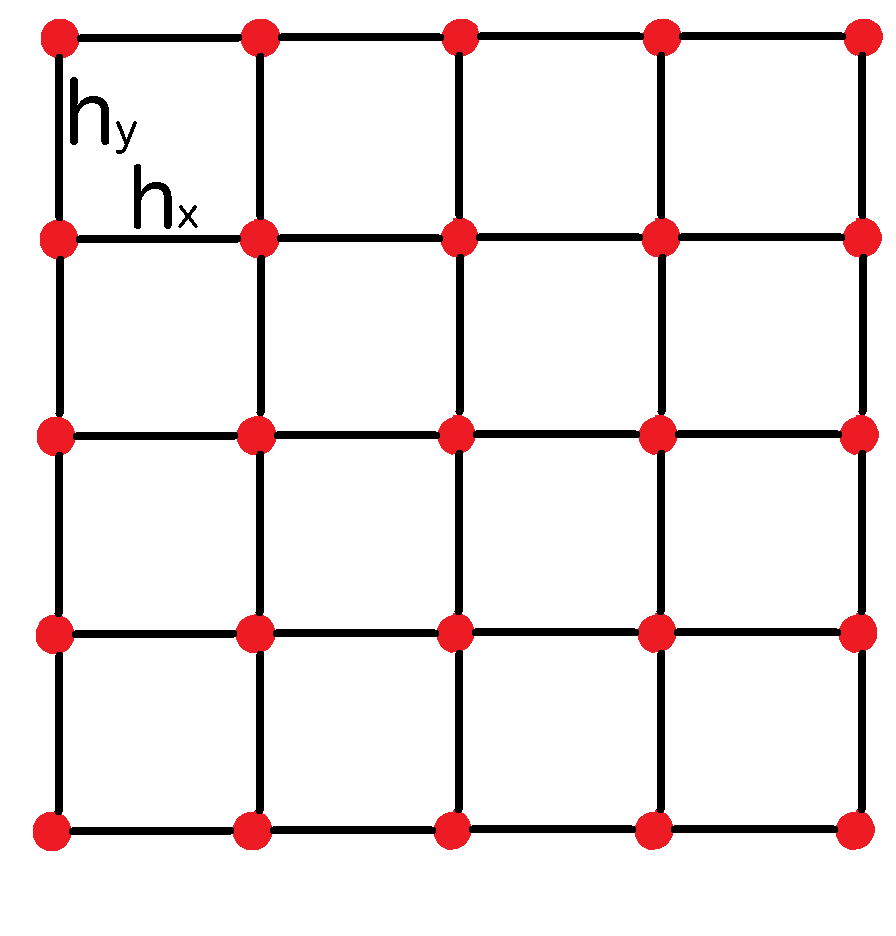
\includegraphics[width=0.90\textwidth]{./images/problems/lect03_computing_grid2d.png}
   \end{center}
  \end{column}
  \begin{column}{0.75\textwidth}
    Now, consider a uniform mesh (grid), as shown on the left,
    where the spacing between neighbouring points along x is h$_x$
    and the spacing between neighbouring points along y is h$_y$.\\
    \vspace{0.2cm}
    Using the {\em first central difference approximation},
    the Laplace equation for any point on the 2-D grid can be written as:
  \end{column}
\end{columns}

\begin{equation*}
   \frac{V(x+h_x,y) - 2V(x,y) + V(x-h_x, y)}{h_x^2} +
   \frac{V(x,y+h_y) - 2V(x,y) + V(x, y-h_y)}{h_y^2} = 0
\end{equation*}

If the grid is uniform (h$_x$ = h$_y$ = h), then the above equation becomes:
\begin{equation*}
   V(x+h,y) + V(x-h, y) +
   V(x,y+h) + V(x, y-h) - 4V(x,y) = 0
\end{equation*}

You have a set of such equations, one for each grid point, which you need
to {\bf solve simultaneously} in order to determine V(x,y) for each grid point.
}
\end{frame}


} % programming

% ------------------------------------------------------------------------------
% ------------------------------------------------------------------------------
